\documentclass{beamer}

% Encoding and language support
\usepackage[T2A]{fontenc}
\usepackage[utf8]{inputenc}
\usepackage[russian]{babel}

% Packages for math and graphics
\usepackage{amsmath}
\usepackage{graphicx}
\usepackage{booktabs} % For better tables
\usepackage{ragged2e} % For text alignment

% Minimalist theme
\usetheme{default}

% Black-and-white color scheme
\setbeamercolor{background canvas}{bg=white}
\setbeamercolor{normal text}{fg=black}
\setbeamercolor{title}{fg=black}
\setbeamercolor{author}{fg=black}
\setbeamercolor{date}{fg=black}
\setbeamercolor{frametitle}{fg=black}
\setbeamercolor{itemize item}{fg=black}
\setbeamercolor{itemize subitem}{fg=black}
\setbeamercolor{enumerate item}{fg=black}

\setbeamertemplate{title page}{
	\vspace*{0.5cm}
	\begin{center}
		
\includegraphics[height=1.1cm]{logo.jpg} % Логотип (можно удалить)
		\vskip0.5cm
		
		{\usebeamerfont{title}\bfseries\large\inserttitle\par}
		\vskip0.8cm
		
		{\usebeamerfont{author}\small
			\textbf{Кромачев М.А.}, гр. 5030102/10201\par}
		\vskip0.3cm
		
		{\usebeamerfont{institute}\footnotesize
			СПбПУ Петра Великого\par
			Физико-механический институт\par}
		\vskip0.8cm
		
		{\usebeamerfont{date}\footnotesize
			Научный руководитель: доц., к.ф.-м.н. И.Е. Ануфриев\par
			\insertdate\par}
	\end{center}
}

% Custom frame title without numbers
\setbeamertemplate{frametitle}{
	\vspace*{0.3cm}
	\begin{beamercolorbox}[wd=\textwidth]{frametitle}
		\usebeamerfont{frametitle}\insertframetitle
	\end{beamercolorbox}
	\vspace*{0.2cm}
}

% Add page number in bottom right corner (except title page)
\setbeamertemplate{footline}{
	\ifnum\insertframenumber=1\else% Skip title page
	\hfill\scriptsize\insertframenumber/\inserttotalframenumber\hspace*{0.5cm}\vspace{0.5cm}
	\fi%
}

% Itemize style
\setbeamertemplate{itemize item}{\color{black}$\bullet$}
\setbeamertemplate{itemize subitem}{\color{black}$\circ$}

% Text alignment
\setbeamertemplate{blocks}[rounded][shadow=false]
\justifying

% Remove navigation symbols
\setbeamertemplate{navigation symbols}{}

\title{Децентрализованное решение задачи о назначениях целей группе роботов}
\author{}
\date{\today}

\begin{document}
	
	\begin{frame}[plain]
		\titlepage
	\end{frame}
	
	\begin{frame}
		\frametitle{Сущность задачи}
		\begin{columns}[T] % Параметр T выравнивает колонки по верху
			\begin{column}{0.5\textwidth} % Левая колонка (текст)
				\begin{itemize}
					\item Цели
					\item Роботы
					\begin{itemize}
					\item Радиус связи
					\item Область видимости
					\end{itemize}
					\item Центр управления
					\item Погрешность определения координат целей
				\end{itemize}
			\end{column}
			\begin{column}{0.5\textwidth} % Правая колонка (изображение)
				\centering
				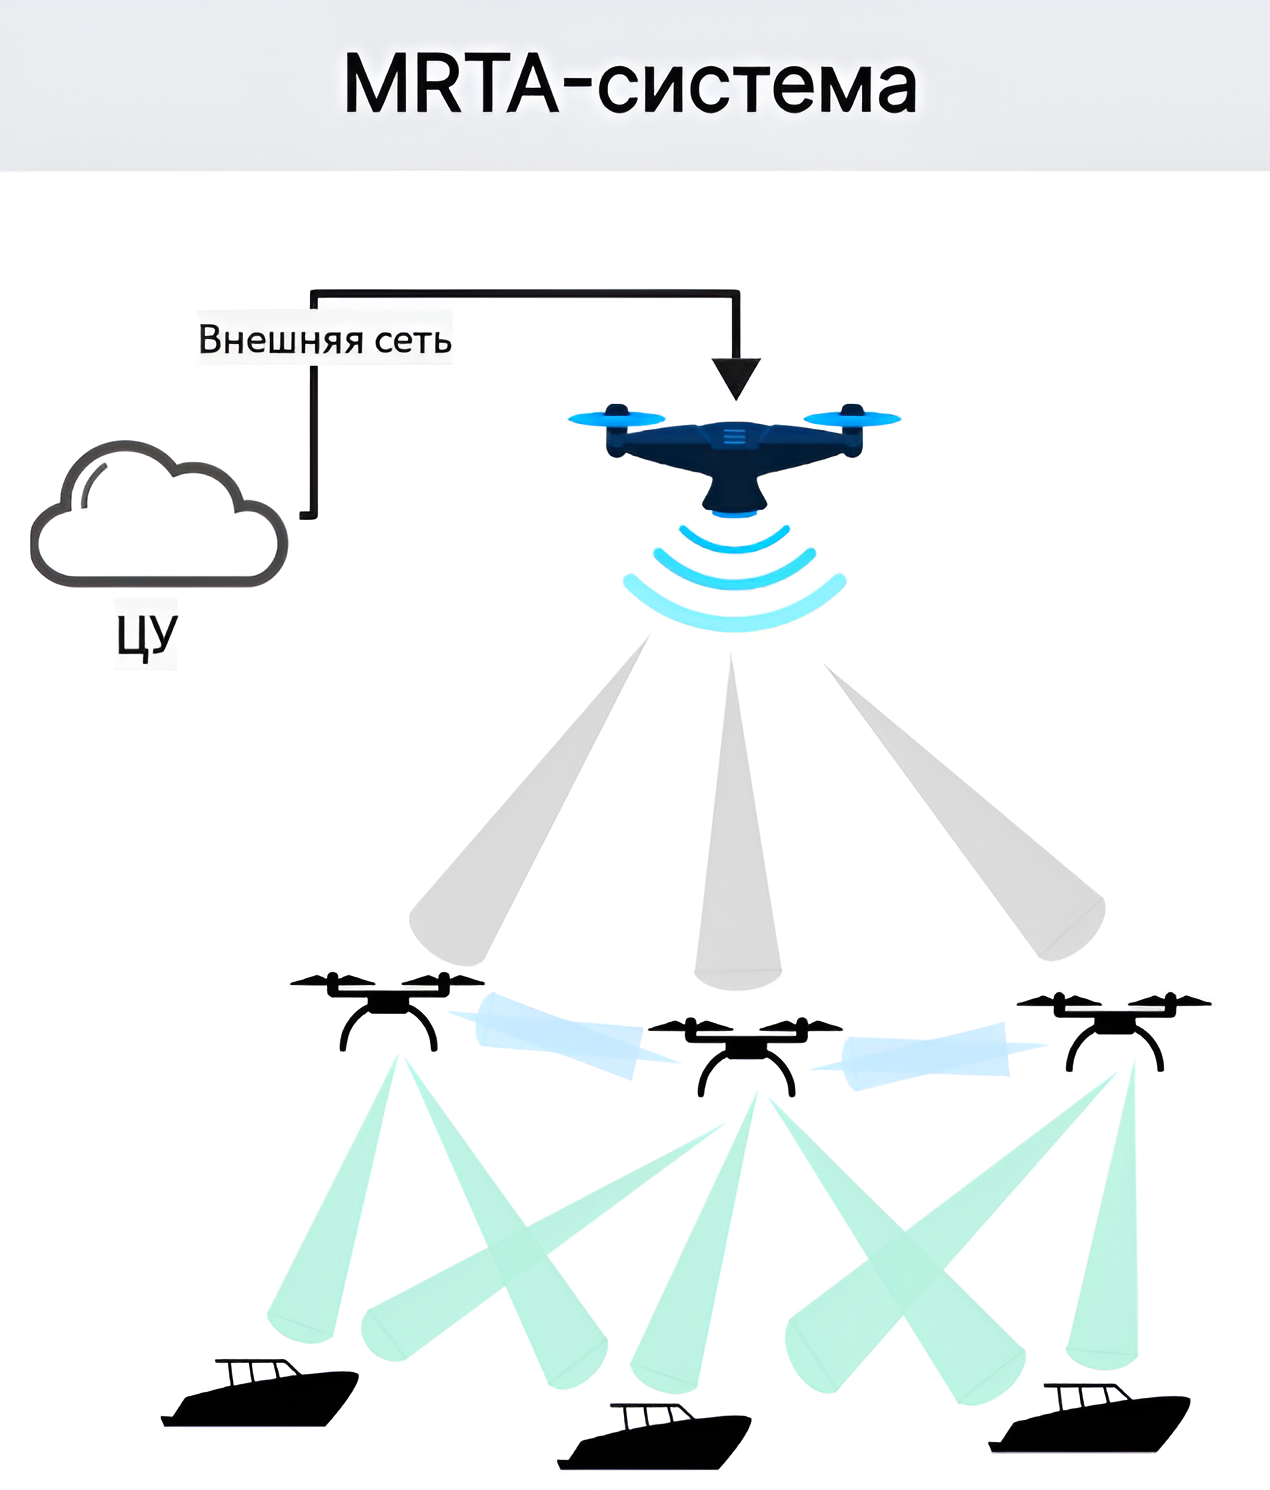
\includegraphics[width=\textwidth,height=0.85\textheight,keepaspectratio]{mrta1.png}
			\end{column}
		\end{columns}
	\end{frame}

	\begin{frame}
		\frametitle{Обзор возможных MRTA-систем}
		\centering
		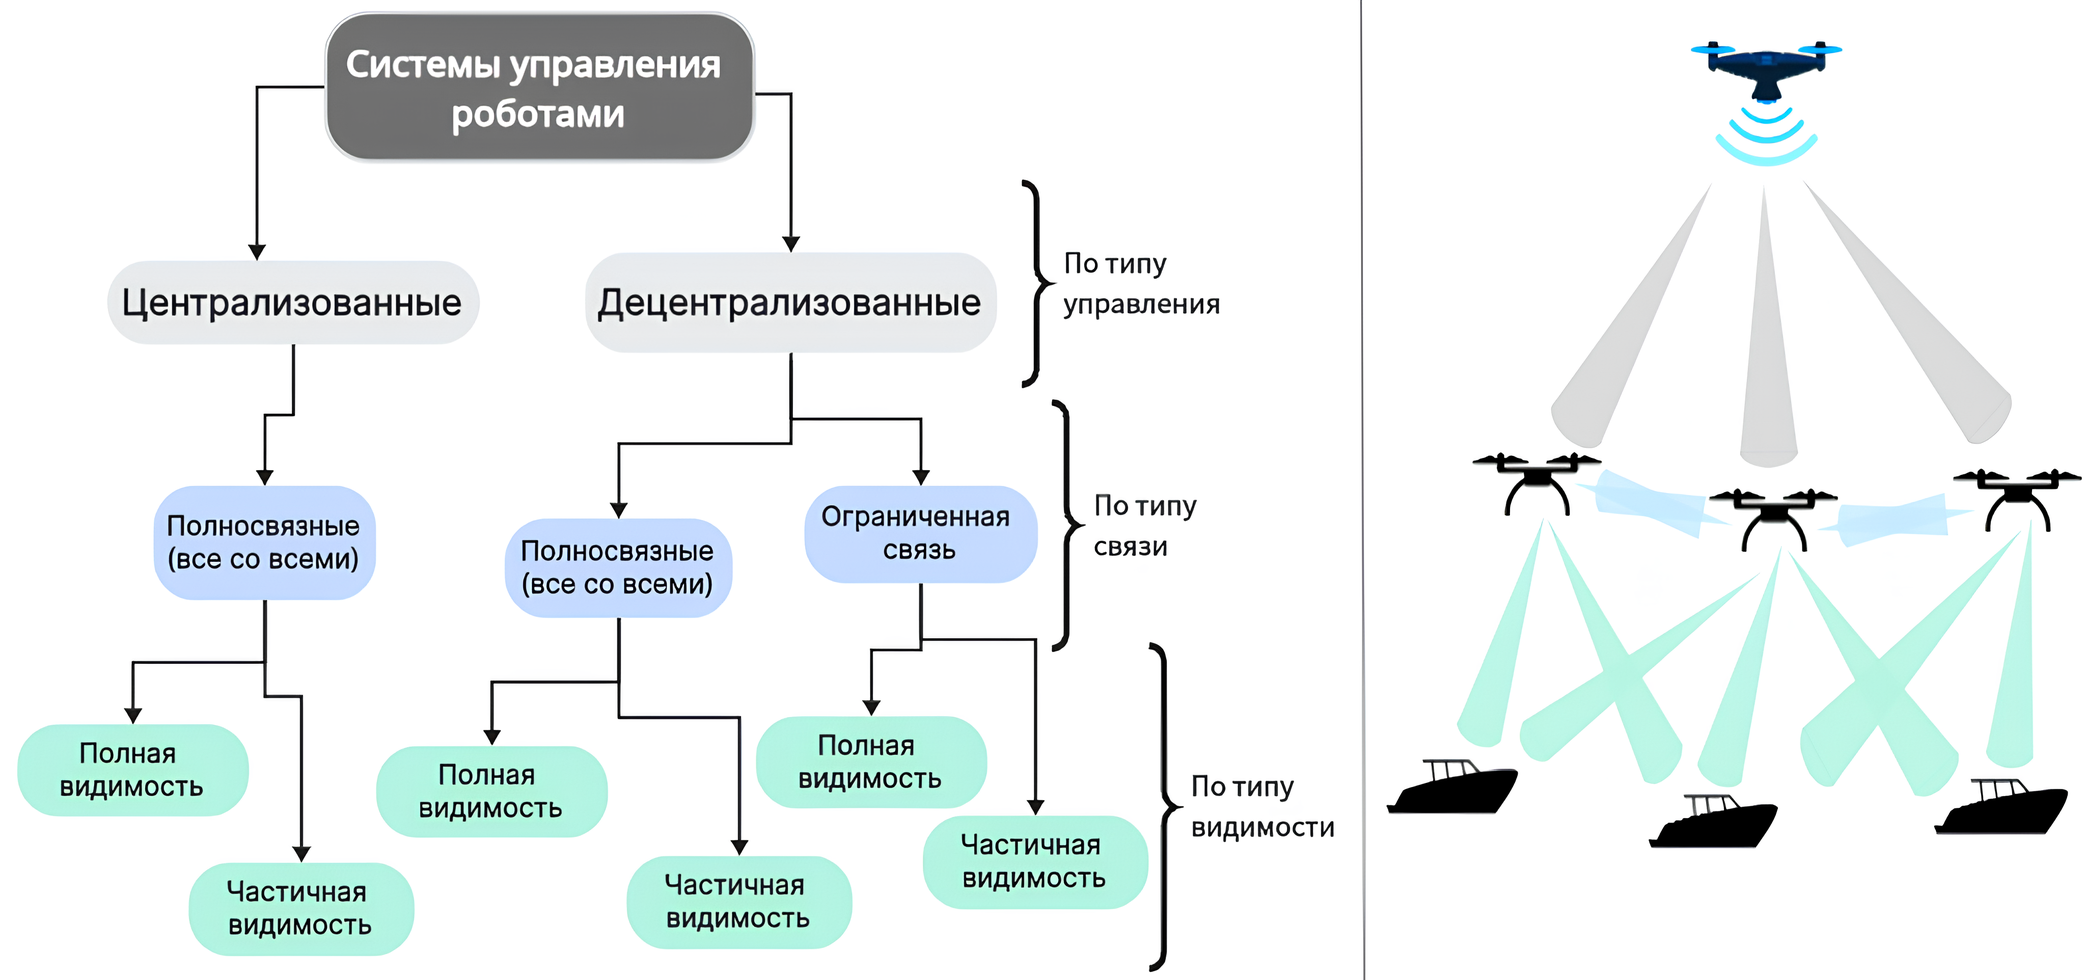
\includegraphics[width=\textwidth,height=0.95\textheight,keepaspectratio]{classification.png}
	\end{frame}


	\begin{frame}
		\frametitle{Положения, выносимые на защиту}
		\begin{itemize}
			\item Итерационный децентрализованный алгоритм назначения целей роботам
			\item Учет ограничения связи (R) и позволяющий управлять точностью решения через параметр (\(\varepsilon\)).
			\item В алгоритме приняты следующие ключевые допущения:
				\begin{itemize}
					\item все роботы имеют одинаковый и неизменный радиус связи
					\item все роботы обладают одинаковыми скоростями движения
				\end{itemize}
			\item Доказано, что алгоритм завершается за конечное число итераций, при этом учет погрешностей измерений обеспечивается адаптивным выбором параметра $\varepsilon$..
			\item Проведено сравнительное исследование, позволившее определить требования к:
			\begin{itemize}
				\item вычислительным мощностям (скорость обработки данных)
				\item каналам связи (скорость обмена информацией)
			\end{itemize}
			при которых модифицированный алгоритм превосходит по эффективности классический венгерский метод.
		\end{itemize}
	\end{frame}

	\begin{frame}{Формальная постановка задачи}
		
		\small
		\textbf{Дано:}
		\begin{itemize}
			\item Множество роботов $R = \{r_1, r_2, \ldots, r_n\}$.
			\item Множество целей $T = \{t_1, t_2, \ldots, t_m\}$.
			\item Матрица выгод $A = \{\alpha_{ij}\}$, где $\alpha_{ij}$ --- выгода от назначения робота $i$ цели $j$.
		\end{itemize}
		
		\textbf{Цель:} Максимизировать суммарную выгоду
		\[
		\sum_{i=1}^n \alpha_{i j_i} \rightarrow \max,
		\]
		где $j_i$ --- цель, назначенная роботу $r_i$.
		
		\textbf{Ограничения:}
		\begin{itemize}
			\item Каждый робот получает не более одной цели: $\sum_{j=1}^m x_{ij} \leq 1, \ \forall i = 1, \ldots, n$.
			\item Каждая цель назначается не более чем одному роботу: $\sum_{i=1}^n x_{ij} \leq 1, \ \forall j = 1, \ldots, m$.
			\item $x_{ij} \in \{0, 1\}$, где $x_{ij} = 1$, если робот $i$ назначен цели $j$, иначе $x_{ij} = 0$.
		\end{itemize}
	
	\end{frame}

	

	\begin{frame}
		\frametitle{Венгерский метод}
		\begin{columns}[T] % Параметр T выравнивает колонки по верху
			\begin{column}{0.4\textwidth} % Левая колонка (текст)
				\begin{itemize}
					\item Единый центр управления
					\item Характеристики радиуса связи можно не учитывать
					\item Полная область видимости
				\end{itemize}
			\end{column}
			\begin{column}{0.6\textwidth} % Правая колонка (изображение)
				\centering
				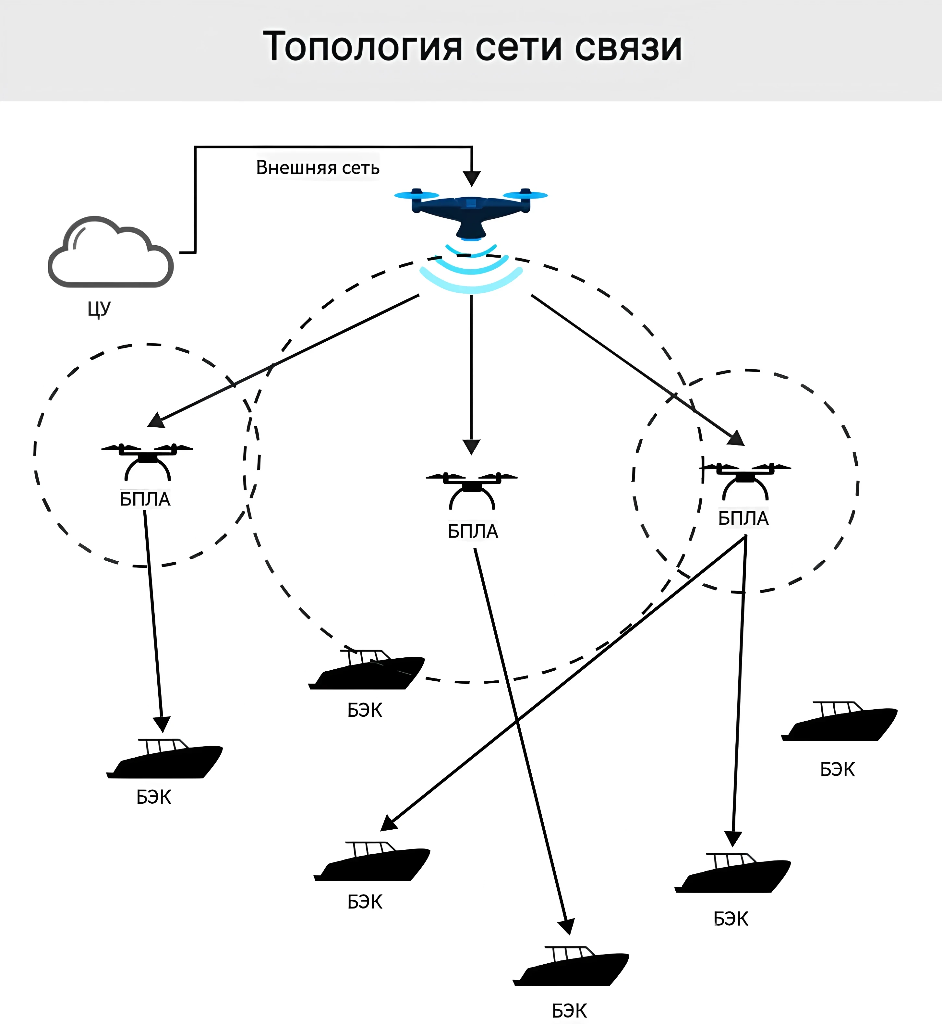
\includegraphics[width=\textwidth,height=0.85\textheight,keepaspectratio]{topology_veng.png}
			\end{column}
		\end{columns}
	\end{frame}

	\begin{frame}
		\frametitle{Алгоритм аукциона}
		\begin{columns}[T] % Параметр T выравнивает колонки по верху
			\begin{column}{0.4\textwidth} % Левая колонка (текст)
				\begin{itemize}
					\item Нет единого центра управления
					\item Требуется полная связь между роботами
					\item Полная область видимости
				\end{itemize}
			\end{column}
			\begin{column}{0.6\textwidth} % Правая колонка (изображение)
				\centering
				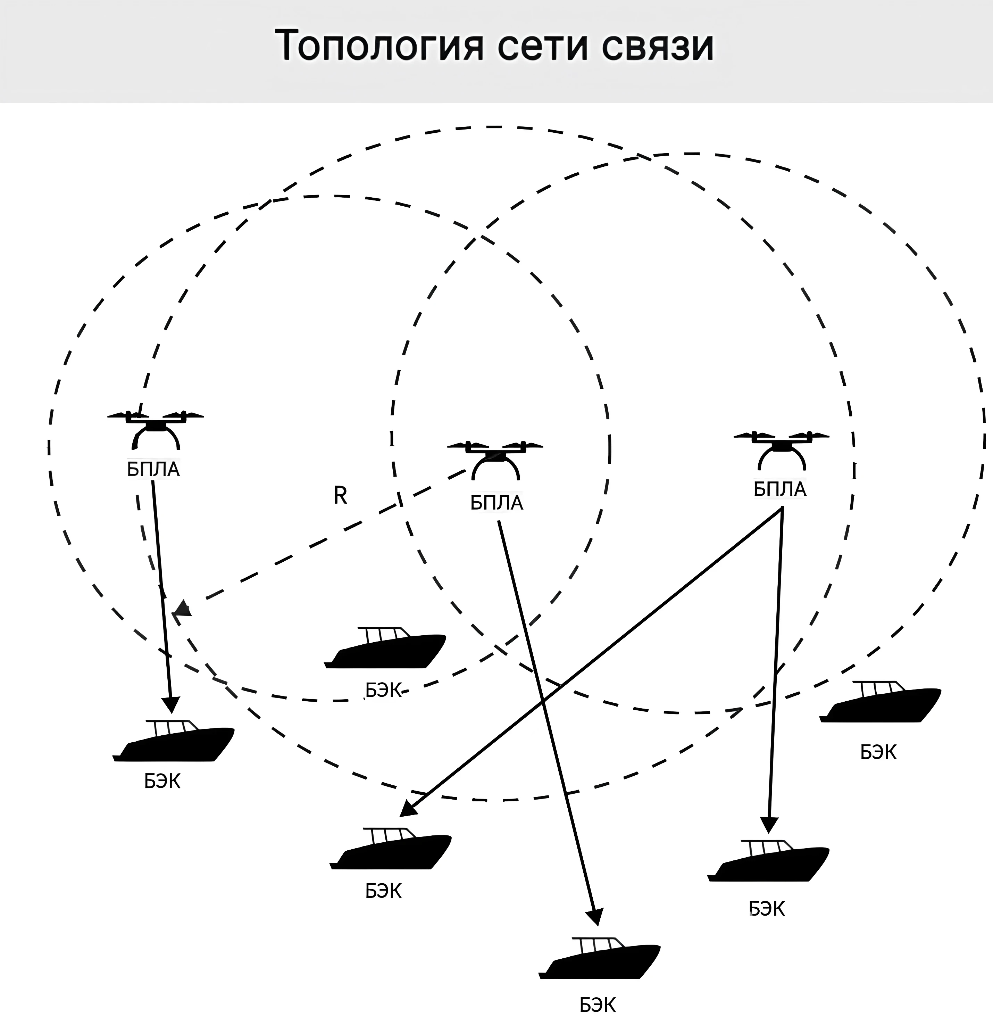
\includegraphics[width=\textwidth,height=0.85\textheight,keepaspectratio]{topology_auction.png}
			\end{column}
		\end{columns}
	\end{frame}

	\begin{frame}
		\frametitle{Модификация алгоритма аукциона}
		\begin{columns}[T] % Параметр T выравнивает колонки по верху
			\begin{column}{0.4\textwidth} % Левая колонка (текст)
				\begin{itemize}
					\item Нет единого центра управления
					\item Требуется полная связь между роботами
					\item Полная область видимости
				\end{itemize}
			\end{column}
			\begin{column}{0.6\textwidth} % Правая колонка (изображение)
				\centering
				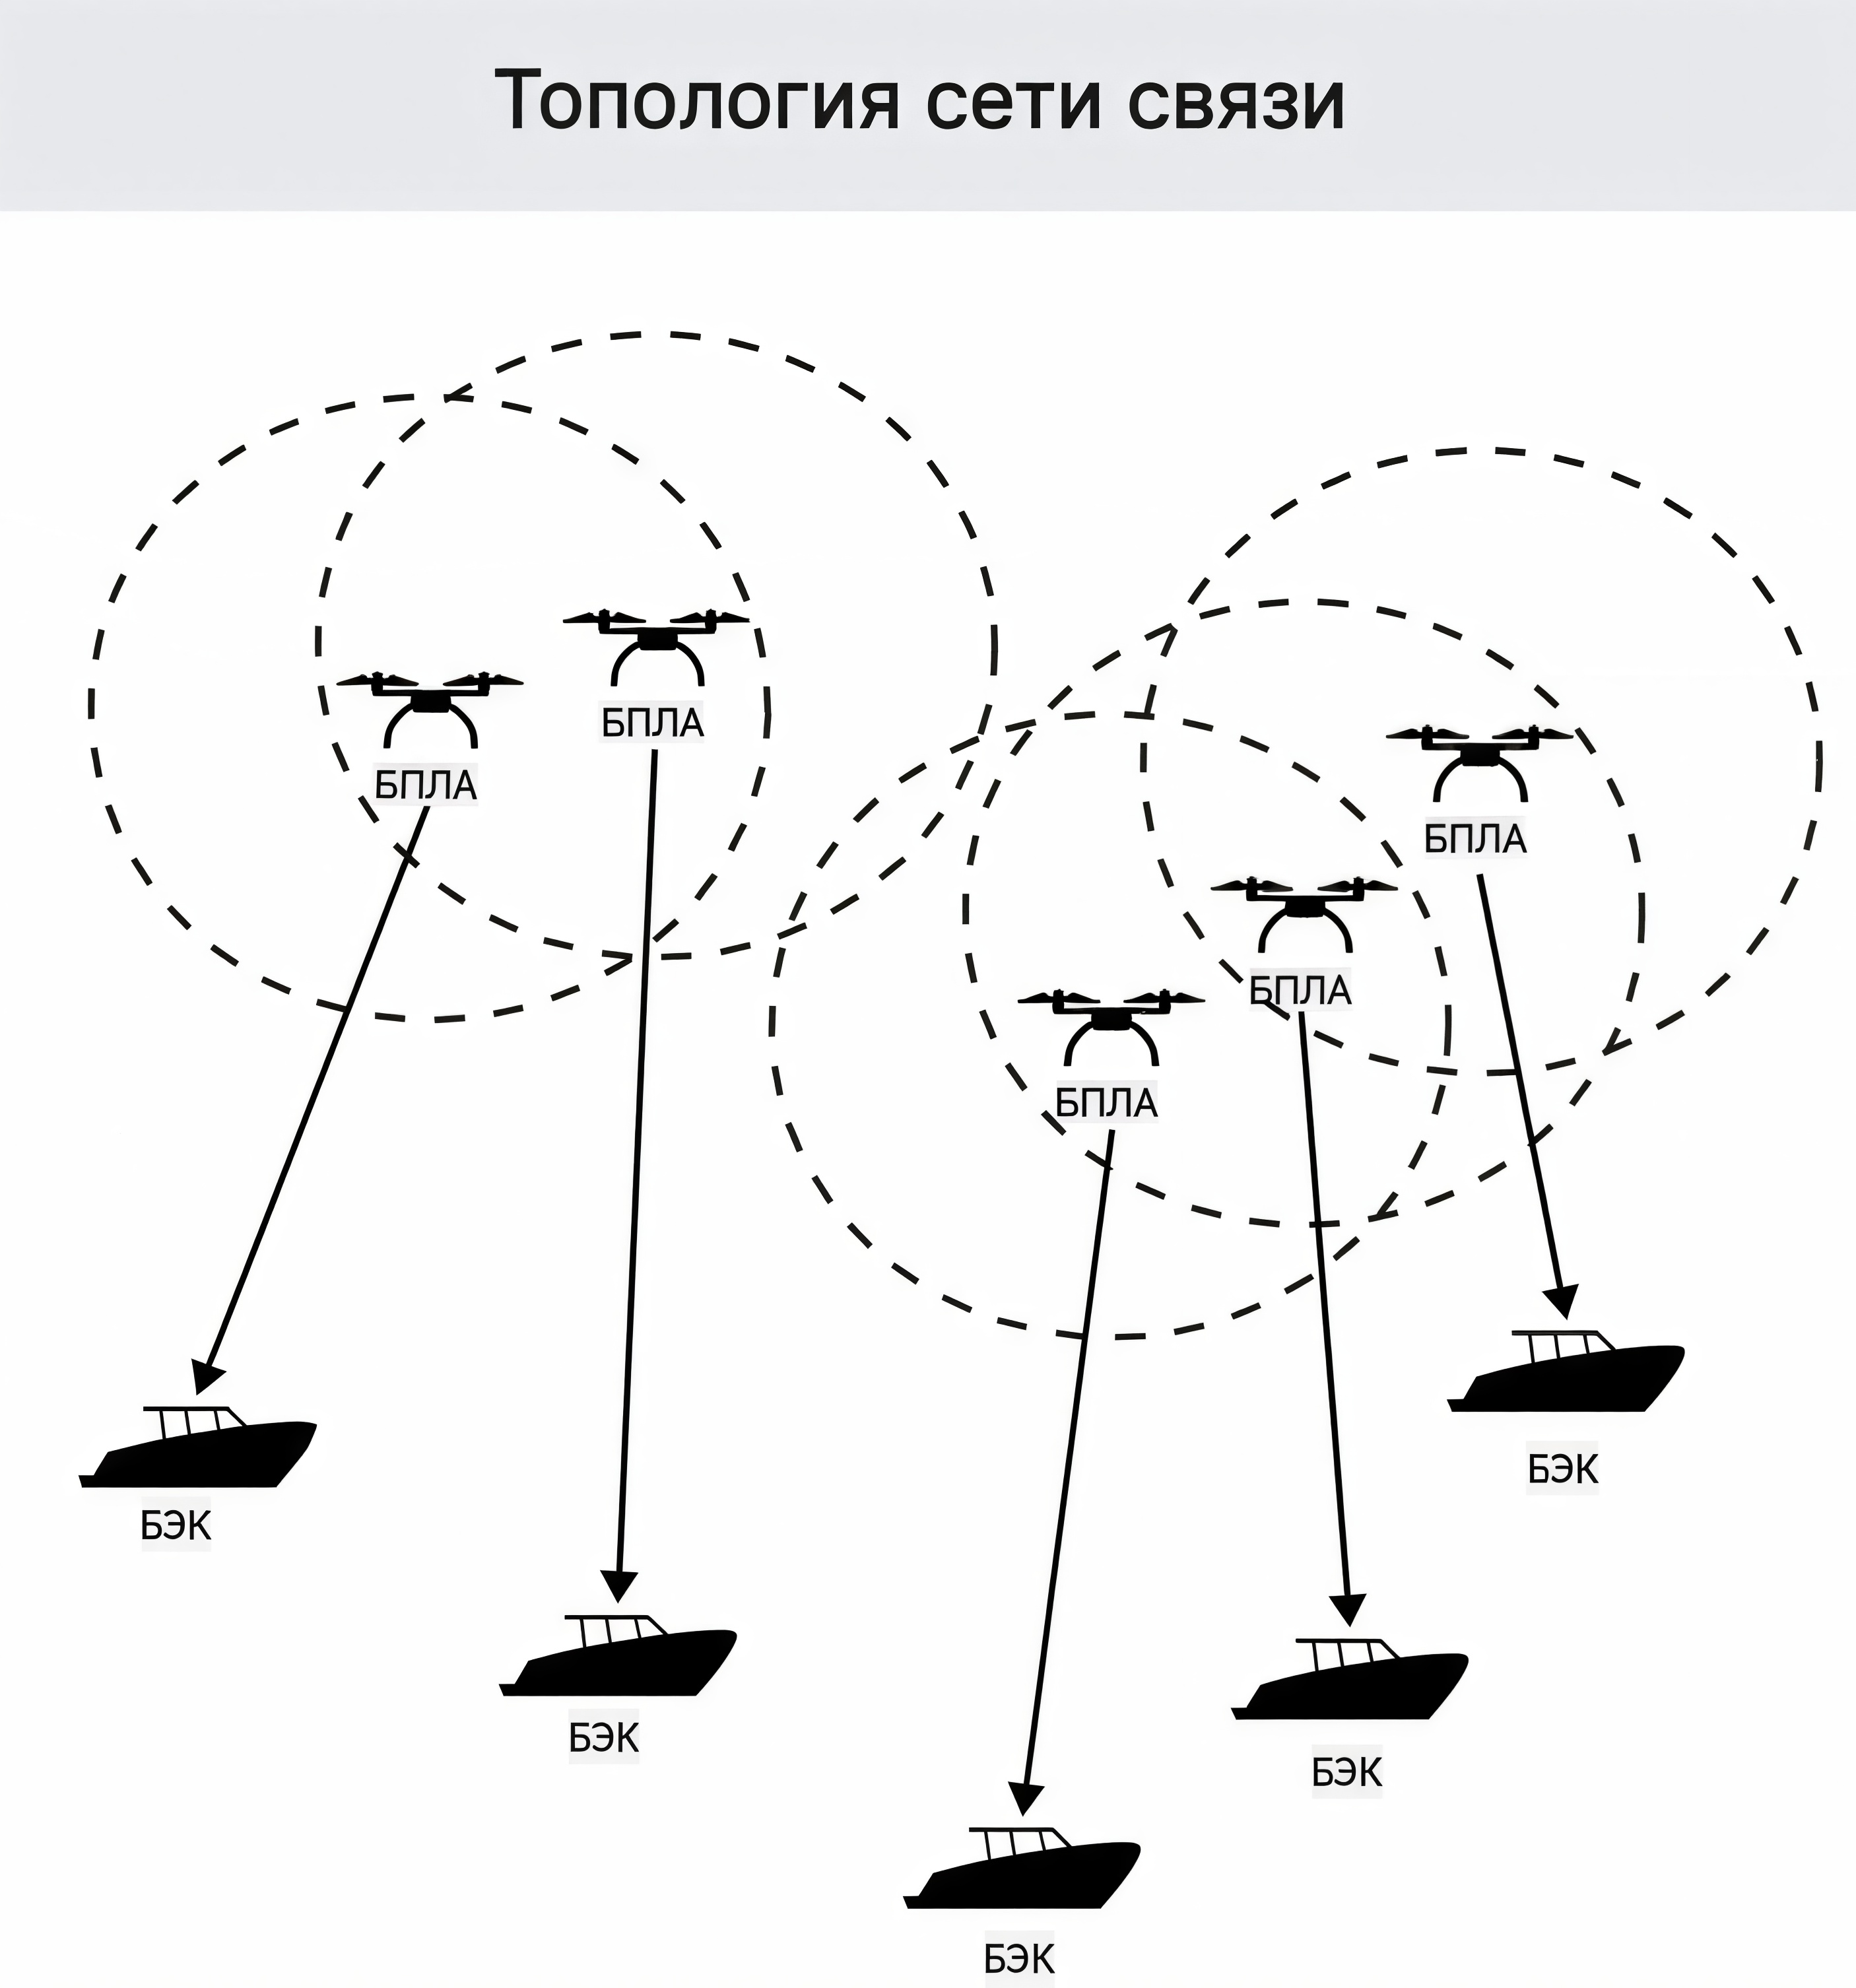
\includegraphics[width=\textwidth,height=0.85\textheight,keepaspectratio]{topology_mod_auct.png}
			\end{column}
		\end{columns}
	\end{frame}
	
	\begin{frame}
		\frametitle{Результаты экспериментов}
	\end{frame}
	
	\begin{frame}
		\frametitle{Выводы и перспективы}
		\begin{block}{Основные результаты}
			\begin{itemize}
				\item Разработан модифицированный аукционный алгоритм
				\item Доказана сходимость и локальная оптимальность
				\item Эффективность подтверждена экспериментально
			\end{itemize}
		\end{block}
		
		\begin{block}{Перспективы развития}
			\begin{itemize}
				\item Улучшение глобальной оптимальности
				\item Адаптация к динамическим сетям
				\item Применение в промышленных системах
			\end{itemize}
		\end{block}
	\end{frame}
	
\end{document}